\chapter{Conclusion}
\label{chap:conclusion}

\section{Summary}

This thesis describes work on several projects involved in the identification and comparison of bacterial ncRNA genes, using homology search and comparative transcriptomics (outlined in Figure \ref{fig:conclusion_methods}). These genes are considerably more difficult to study than their proteinaceous bretheren, as they lack obvious genomic signals such as stop/start codons, and features such as their short length and flexible requirements for function allow ncRNA nucleotide sequences to change rapidly over a small span of evolutionary time. 

The potential reasons for this observation are reviewed in Chapter 2, in which the relative probabilities ncRNA gene acquisition due to \textit{de novo} gene formation, exaptation and horizontal gene transfer are considered. In Chapter 3, we asked if this observation is due to the limitations of pairwise sequence alignment-based homology search methods. We developed a homology search pipeline based on iterative profile HMM approach, which incorporated signals of synteny, to study the conservation of \textit{Salmonella} Typhimurium sRNAs. Manual predictions of sRNA origins, using signals of sRNA conservation and the function of nearby genes   identified a clear picture of the reasons for sRNA gene gain and loss in \textit{Salmonella}. This work outlines a sensitive pipeline for annotating highly diverse sRNA sequences, and also identified sequence features of sRNAs which are likely to return high numbers of false positives. 

Transcriptome data for an economically-relevant pathogen, \textit{P. syringae} pv. \textit{actinidiae} grown \textit{in vitro}, was generated for this project, primarily for the aim of identifying ncRNAs relevant to virulence. In Chapter 4, gene expression \textit{in vitro} in multiple growth conditions was compared to data generated \textit{in planta}, as well as the literature. This showed that the \textit{in vitro} data captures major responses to nutrient stress, namely the production of siderophores in nutrient-depleted conditions, and under starvation conditions the activation of metabolic adaptions to alternative carbon sources, as well as expression of virulence genes involved in adhesion, defence against plant defence molecules and physiological stress.

Visualisations of \textit{in vitro} and \textit{in planta} transcriptomes were then used to guide the annotation of novel ncRNAs expressed in \textit{Psa}. The homology search pipeline developed for Chapter 3 was applied to identify conserved candidates and generate multiple sequence alignments, which were used to look for signals of secondary structure conservation that are likely to indicate function.

Chapter 6 describes work on a genome assemblies of five genomes of the genus \textit{Gemmata}. Preliminary analysis of these genomes identified that these isolates have diverse genome structures and high density of mobile genetic elements. This is part of a larger work aiming to generate genomes and transcriptomes for between-phyla comparison of intergenic expressed regions to identify conserved and expressed intergenic regions indicative of functional ncRNAs. 
\subsection{Where do sRNA genes come from?}

We first considered the current literature surrounding sRNA evolution, which suggests that sRNAs are likely to be rapidly gained and and lost, and exhibit high sequence turnover. In our review, we considered the potential reasons for gene gain and loss, as the small size and minimal functional requirements for an sRNA make them attractive models for observing or modelling \textit{de novo} gene evolution. We also explored the relative likelihood of different routes to \textit{de novo} gene evolution, \textit{via} the capture of stochastic transcription of intergenic regions, termed 'transcriptional noise'. 

To explore if this observation is due to the limitations of pairwise sequence alignment-based homology search methods, we developed a pipeline based on iterative profile HMM searches, aiming to accurately identify highly divergent homologues from single sequences.

\newpage
\begin{figure}[H]
    \centering
    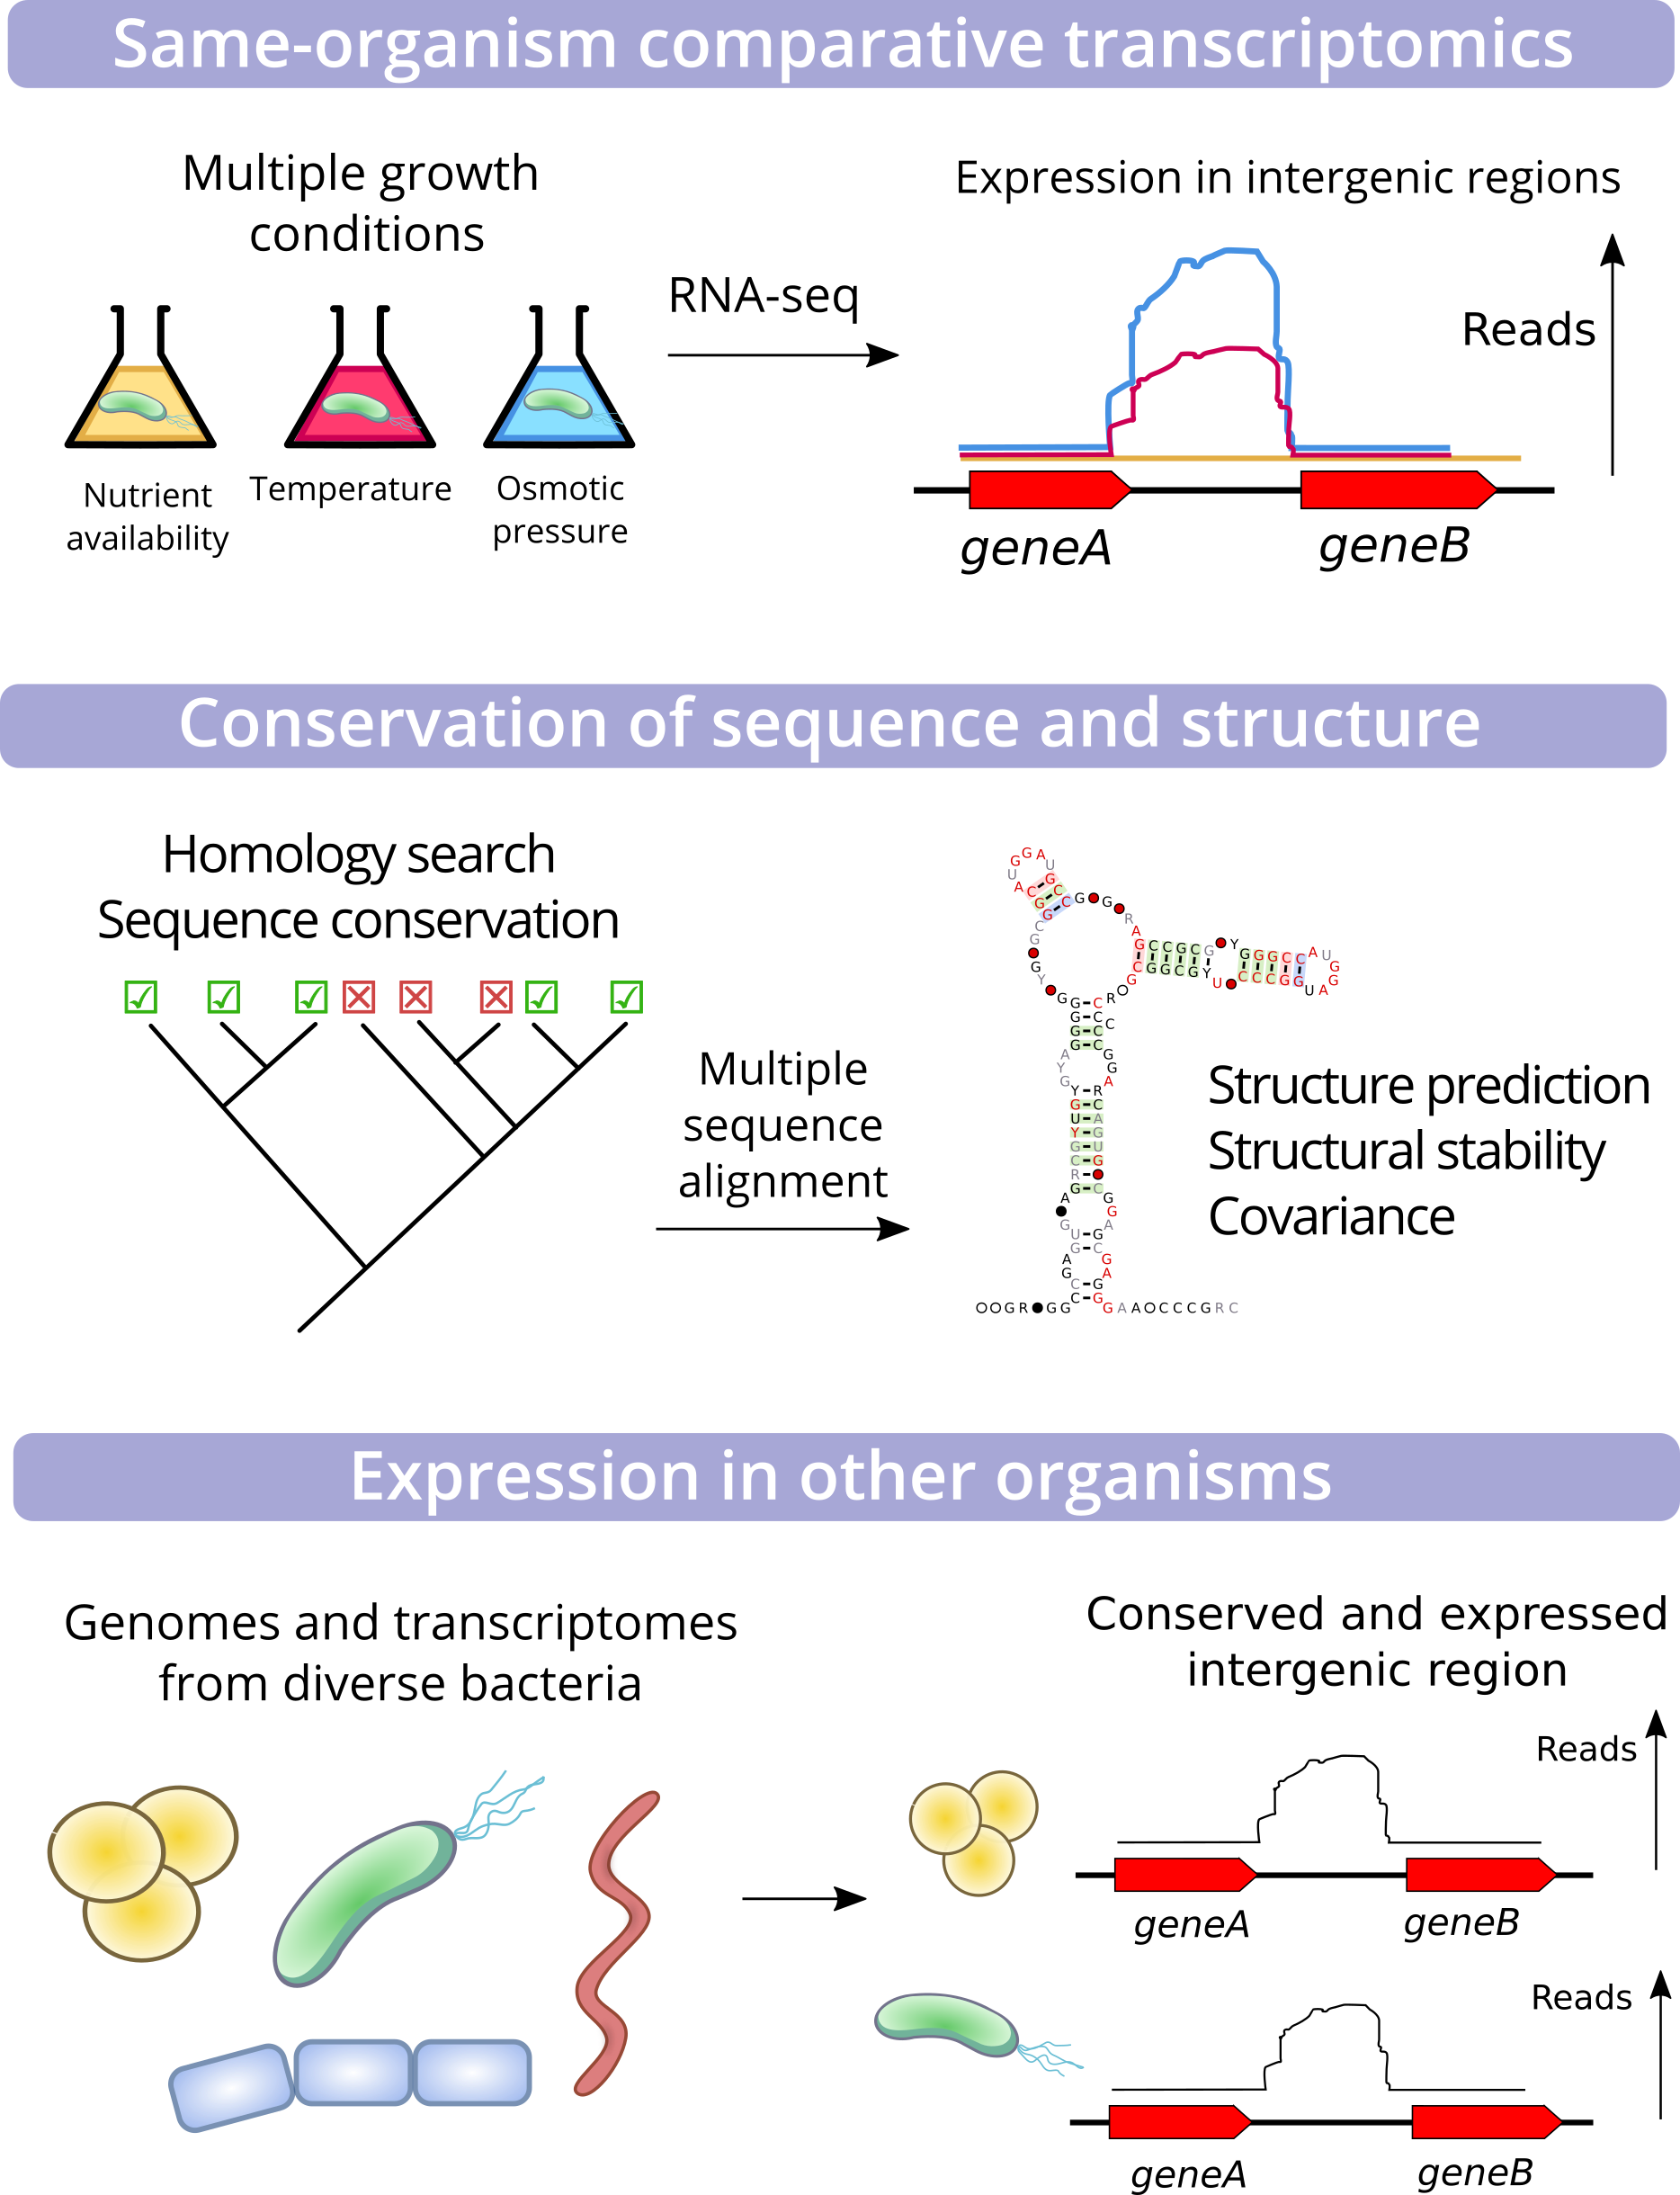
\includegraphics[scale=0.9]{other/ways_to_find_ncRNAs.png}
    \caption[Methods for the identification of ncRNAs used in this thesis]{Methods for the identification of ncRNAs used in this thesis. Top: Same-organism comparative transcriptomics, where a single strain is grown in multiple growth conditions to identify condition-specific ncRNA expression in intergenic regions (Chapter 5). \textbf{Middle:} Conservation of sequence and structure, using homology search to study the sequence conservation of ncRNAs (Chapter 3). This can then be used to identify structure conservation, which may be used to improve homology search or as an indicator of function for candidate ncRNAs (Chapter 5). \textbf{Bottom:} Expression in other organisms, where the conservation of expression homologous sequences can be used as a signal of function (Chapter 5), particularly over large phylogenetic distances (Chapter 6). }
    \label{fig:conclusion_methods}
\end{figure}

We focused on intergenic ncRNAs, which we would expect to be more free to rapidly evolve than those opposite to, or that have substantial overlap with, protein-coding genes. Allowing for more sequence divergence presented several issues with models for paralogous ncRNAs overlapping with each other, and small sequences with low sequence complexity or similarity to genomic motifs generating highly-multi-copy annotations.

A 3-model approach was implemented, incorporating nearby sequences as synteny anchors. This was effective for resolving annotation conflicts and separating true and false positives. A flanking protein approach was also trialled, did not significantly improve the accuracy of results and was more computationally demanding.

The homology search pipeline has been automated, with a large scale analysis such as in Chapter 3 taking approximately 24hrs with a high-performance desktop computer. This method was also successfully applied to study the conservation of candidate ncRNAs in \textit{Psa}, and which identified a functionally characterised homologue in \textit{P. aeruginosa}. 

\subsection{Methods to identify horizontally-acquired ncRNAs}

Conservation of sRNA sequences and synteny anchors, as well as surrounding gene annotations were used to establish approximate ages and gene origins for \textit{Salmonella} sRNAs. 
The analysis of gene origins was largely exploratory, aiming to identify if poor conservation was due to sequence divergence or the product of horizontal gene transfer. Initially, sRNA genes were classed manually using conservation and gene annotations. A large scale annotation of sRNA flanking proteins was subsequently added to provide a metric for classification. While this was able to distinguish between poorly conserved sRNAs and HGT-associated sRNAs, vertically-inherited sRNAs were also associated with MGE insertions. This was significantly more computationally intensive than the homology search analysis, and required a curated list of protein descriptions associated with mobile genetic elements. In this case, a measurement of conservation and phylogenetic spread may be a simpler way to detect HGT-associated ncRNAs.

Chromosomal MGEs are likely to be a largely unexplored source of ncRNAs, however prokaryotic MGE annotation has lagged behind chromosomal genes \citep{Frost2005-wt}. MGE nomenclature and classification methods are varied \citep{Piegu2015-dq}, and annotation information is often poorly integrated across databases. Early large-scale MGE databases such as ACLAME \citep{Leplae2010-zq} have not been maintained (last update 2013). Other databases are restricted to MGEs in a specific organism or clade \citep{Partridge2018-mh}, or focus on specific MGE types \citep{Arndt2016-hj}. Some poorly understood or diverse classes of MGEs, such as group II introns, also remain difficult to identify without manual curation steps \citep{Candales2012-ws}. 

Automated generalised methods for MGE annotation are emerging, combining homology, repeat-identification and synteny information to find MGEs \citep{Berthelier2018-sd}. As annotation improves, we will be better able identify and study the spread and evolution of ncRNAs associated with MGEs through bacterial lineages.

\subsection{Tracking ncRNAs through bacterial phylogenies}

The study of many ancient ncRNAs and proteins is obfuscated by genetic drift \citep{Hoeppner2012-llpl}. The rapid evolution of bacterial sRNAs may serve as a useful analogous system to test homology search tools designed to study deep time evolutionary processes, as the most rapidly evolving sRNAs have diverged on a timescale over which protein sequences and synteny remain stable. 
Incorporating synteny is a useful way to identify bacterial sRNAs, as nearby protein coding genes are likely to have a slower rate of sequence divergence. In Chapter 3 synteny information also provided an estimate of the conservation of the locus containing an sRNA, which allowed us to identify sRNAs that had diverged beyond sequence alignment. However, this was only found to have occured a small proportion of \textit{Salmonella} sRNAs, and were often caused by insertions rather than significant amount of nucleotide substitutions.

Short nucleotide sequences flanking sRNAs were effective in by providing increasing sensitivity without specificity, allowing the detection of sequences in small homologous MGEs that may not have been detected by using flanking proteins. Many sRNAs were located at sites of recombination or MGE insertion, and the short length of the flanking sequences allowed us to detection of the origin of an MGE after a locus had been disrupted or eroded due to purifying selection. 

Homology search will have varying effectiveness depending on the selection pressures on the sRNA sequence. While structural requirements can be modelled, functional information is difficult to incorporate. We have used expression and observed interactions with RNA-binding proteins as a proxy for regulon size, which appears to restrict sequence conservation. However it is difficult to explore the relationship between sequence divergence and function without additional information in other species for comparison.

%Genomic flexibility and optimisation particularly well demonstrated by \textit{Pseudomonas syringae}, which can be seen by the complex transcriptional restructuring in different growth conditions (Chapters 4 and 5). The identification of candidate regulatory ncRNAs may help further elucidate the regulons which control these responses.

%Non-coding RNA regulation appears to be ubiquitous in bacteria. 
%which predicts that - RNA-based regulation can create complex regulatory circuits from simple evolutionary process/molecules

\subsection{Integrative approaches to gene annotation}

The lack of centralised resource for bacterial ncRNA annotations and function is a limiting factor for doing large-scale comparative studies. Currently, functional information for sRNAs depends on the availability of data-sets in the literature. Rfam \citep{Nawrocki2015-aatt} and RNAcentral \citep{The_RNAcentral_Consortium2019-lf} are well-maintained databases for ncRNA sequence and structural information, however these have limited information about the functions and targets of individual ncRNAs besides literature references. Several attempts have been made to create resources for functionally characterised sRNAs, however at the time of writing these are not currently maintained \citep{Li2013-wl,Huang2009-kk} or are no longer functional \citep{Wang2016-ul,Pischimarov2012-za}. 

Genome annotations for the location and targets of regulatory elements are provided for eukaryotic model organisms in NCBI (https://www.ncbi.nlm.nih.gov/refseq/functionalelements/), ENCODE \citep{ENCODE_Project_Consortium2012-qj} and ensembl \citep{Zerbino2015-fr,Zerbino2016-ak}. Small databases of bacterial transcription factors binding sites such as Prodoric \citep{Eckweiler2018-ay} and collectTF \citep{Kilic2014-md}, have yet to be included as part of prokaryotic annotation pipelines.

\subsection{Dense and varied sampling required to provide power to comparative approaches}

The continued integration of new experimental technologies and computational methods are making the functional characterisation of ncRNAs easier, cheaper and more comprehensive \citep{Georg2019-vl,Stav2019-mr}. Work to generate data-sets in emergent strains of \textit{S.} Typhimurium \citep{Canals2019-xxyv} are to providing insight into how rapidly changes in expression and regulation can occur. 

We have used a complementary experimental and computational approach to identify and rank candidate ncRNAs in \textit{Psa}. However, this analysis was limited as the design of this experiment was not complete, and had variable numbers of replicates. As this restricted the \textit{in vitro} analysis to pairwise comparisons of growth media, growth phase is likely to be a confounding factor in this analysis. Additional replicates in minimal media in other growth phases would help to resolve this issue. The low read depth and unstranded nature of the \textit{in planta} was only able to confirm the expression of highly-expressed transcripts, and it is likely that weakly expressed ncRNA transcripts may have been missed. This is also the case for the \textit{P. syringae} pv. \textit{tabaci}. A replicated experiment in another \textit{Psa} strain or \textit{P. syringae} pathovar, or a same-family outgroup such as \textit{P. fluorescens}, \textit{P. putida} or \textit{P. aeruginosa} would be useful to confirm the expression of homologous sequences, and to identify more novel ncRNAs.

In-host RNA-seq of bacterial pathogens are useful for condition-specific expression of ncRNA genes and regulons important for pathogenicity \citep{Westermann2016-mxr}. A number of experiments have now been performed \textit{in vivo}, including work to explore the changes in both the bacteria and the host. However, these experiments are more difficult to achieve \textit{in planta}, due to the large plant cells, tough cell walls and difficulty in enriching bacterial reads \citep{Nobori2018-ux}. Despite these limitations, we could still identify a variety of expressed candidate ncRNAs in \textit{Psa} grown \textit{in planta}. These data were also useful for confirming the expression of candidate ncRNAs identified using \textit{in vitro} data. 

%-- planctomycetes work as part of work to generate datapoints for transcriptome comparison

\subsection{Future work}

We plan to write a paper based on the work described in Chapter 3, and package the pipeline for wider use. We intend to submit this work to an RNA-focused journal such as Nucleic Acids Research. I also aim to further explore sequence features and conservation patterns that are likely to cause issues with homology search, and to identify genes within mobile genetic elements, to perform the gene origin analysis without large amounts of additional manual curation or increased computational load.  

The analysis of the \textit{Psa} transcriptomes in Chapter 4 and Chapter 5 will also provide the basis for a future publication. This will primarily focus on the \textit{Psa} candidate ncRNAs identified in Chapter 5. Experiments are planned to experimentally verify and functionally characterise these candidates. Of particular interest is the \textit{pesA} homologue present in \textit{Psa}, which has a role in intracellular survival in \textit{P. aeruginosa}. PesA shows different expression patterns in \textit{Psa}, which has a different set of environmental stresses as a plant pathogen. Recent comparisons between Enterobacteriaceae pathogens that infect plant and animal hosts show that conserved sRNAs can acquire lifestyle-specific functions. ArcZ, which is involved in the anaerobic stress response in the gut pathogen \textit{E. coli} K12 \citep{Mandin2010-jf}, also has a function in surviving H\textsubscript{2}O\textsubscript{2} plant defence in \textit{Erwinia carotavora} 
\citep{Schachterle2019-rq}. The change of expression pattern of PesA suggests that a similar process of functional specialisation may have occurred in \textit{Pseudomonas}.

The genome assembly and analysis of the planctomycetes genomes, as well as representatives of the genus \textit{Halococcus} will continue as part of an ongoing collaboration to identify and compare ncRNA expression across wide phylogenetic distances \citep{Lindgreen2014-rmv}.

\section{Concluding statement}

Rapidly developing experimental and computational methods are increasing the power and scope of comparative methods. While the study of pathogens often focuses on the study of protein-coding genes, the presence and function of ncRNAs are increasingly becoming appreciated, as these can effect large-scale changes in gene regulation. The study of mobile genetic elements will likely feature heavily, as larger MGEs such as pathogenicity islands that are important determinants of niche-specificity \citep{Melnyk2019-cclx}, are particularly enriched for sRNA genes.

For those sRNAs which are subject to rapid sequence change, the question remains as to how their regulons evolve and diversify. As conserved ncRNAs with divergent sequences can have conserved functions \citep{Horler2009-vava}, the comparison of rapidly-diversifying sRNAs may provide insight into the relationships between structure, sequence and function can co-evolve. Our increased ability to understand the function and essentiality of these genes will facilitate such studies.

Further work is needed to explore whether the rapid gene gain and loss of sRNAs occurs outside of fast-evolving pathogen species, or in less well-studied phyla. Using a starting point outside of the \textit{Salmonella}-\textit{Escherichia} lineage would be interesting to see if homology search annotations from different phylogenetic starting points shows similar patterns of conservation. Comparisons of sRNA conservation in other families, such as Pseudomonas, Streptococcus, Staphylococcus or Mycobacteria. The data-sets generated in \textit{Psa} provide a comprehensive starting point for such a study, similar to the \textit{S.} Typhimurium data-set by \citep{Kroger2013-pppg} used in Chapter 3. 


%mge-associated ncrnas - the discovery of ncRNAs which interfere with eukaryotic transcription may be an especially interesting area as their targets are more likely to be stable
%http://dx.doi.org/10.1128/mBio.01223-19 (opp transposase https://rfam.org/family/rli32).. check if in known mge/islands here? https://bmcgenomics.biomedcentral.com/articles/10.1186/1471-2164-14-47

%maybe pinT also
\bibliographystyle{otago}
\bibliography{conclusion}